\documentclass[12pt, a4paper, oneside, titlepage]{report}

\usepackage{ngerman}
\usepackage[utf8]{inputenc}
\usepackage[T1]{fontenc}
\usepackage{latexsym}
\usepackage{amsmath,amsfonts,amssymb,amsthm,amscd}
\usepackage{dsfont}
\usepackage{graphicx}
\usepackage[flushleft]{paralist} 
\usepackage[dvipsnames]{xcolor} 
\usepackage[all]{xy}
\usepackage{makeidx}
\usepackage{graphicx}
\usepackage{verbatim}
\usepackage[numbers]{natbib} % [numbers,round]

\usepackage{pgf}
\usepackage{tikz}
\usepackage{pgfplots}
\usepackage{mathrsfs}
\usepackage{adjustbox}
\usepackage{float}

% \usepackage{showframe}

\usetikzlibrary{arrows}
\pgfplotsset{compat=1.15}

\usepackage{url}
\usepackage{hyperref}

\newcommand{\R}{\mathds{R}}
\newcommand{\Z}{\mathds{Z}}
\newcommand{\N}{\mathds{N}}
\newcommand{\Q}{\mathds{Q}}
\newcommand{\K}{\mathds{K}}
\newcommand{\C}{\mathds{C}}
\newcommand{\B}{\mathds{B}}
\newcommand{\F}{\mathds{F}}
\newcommand{\p}{\mathfrak{p}}
\newcommand{\Pot}{\mathcal{P}}
\newcommand{\id}{\textup{id}}
\newcommand{\Ker}{\textup{Ker}}
\newcommand{\Image}{\textup{Im}}
\newcommand{\la}{\langle}
\newcommand{\ra}{\rangle}

\newtheorem{lemma}{Lemma}[section]
\newtheorem{prop}[lemma]{Proposition}
\newtheorem{defprop}[lemma]{Definition and Proposition}
\newtheorem{satz}[lemma]{Satz}
\newtheorem{thm}[lemma]{Theorem} 
\newtheorem{kor}[lemma]{Korollar} 
\newtheorem{folg}[lemma]{Folgerung}
\newtheorem{verm}[lemma]{Vermutung}
\newenvironment{bew}{\begin{proof}[Beweis]}{\end{proof}}
\theoremstyle{definition} 
\newtheorem{def1}[lemma]{Definition} 
\newtheorem{bem}[lemma]{Bemerkung}
\newtheorem{ford}[lemma]{Forderung}
\newtheorem{bsp}[lemma]{Beispiel}
\newtheorem{notation}[lemma]{Notation}

\renewcommand\thesection{\arabic{section}}

\author{Henning Hontheim}
\title{Secret Sharing}
\date{10. März 2020}

\let\svthefootnote\thefootnote
\newcommand\blankfootnote[1]{%
	  \begin{NoHyper}
	  	\let\thefootnote\relax\footnotetext{#1}%
	  	\let\thefootnote\svthefootnote%
	  \end{NoHyper}
}

\setcounter{tocdepth}{3}

\begin{document}
	\begin{titlepage}
		\maketitle
		\thispagestyle{empty}
		\pagenumbering{Alph}
		\tableofcontents
		\thispagestyle{empty}
		\blankfootnote{Allein aus Gr"unden der Lesbarkeit wird auf die gleichzeitige Verwendung mehrerer geschlechtsspezifischer Sprachformen verzichtet. S"amtliche Personenbezeichnungen gelten f"ur alle Geschlechter.}
		\clearpage
	\end{titlepage}
	\pagenumbering{arabic}

	\section{Wozu Secret Sharing?}
	Arbeiten Sie mit Anderen an einem geheimen Projekt, so gibt es einige Herausforderungen zu meistern. Was passiert, wenn Sie Ihren Schlüssel der verschlüsselten Daten verlieren? Haben lediglich Sie einen Schlüssel? Wahrscheinlich nicht. Es ist nützlich, seien es in einem Tresor verschlüsselte Daten, oder die privaten Schlüssel in einer PKI, wenn nicht nur Sie den einzigen Schlüssel besitzen.
	
	Aber wie teilen Sie den Zugriff auf die Daten? Wenn Sie Ihren Schlüssel vervielfältigen würden, hätte ein Einzelner Vollzugriff. Es wäre besser, wenn es mehrere Personen benötigen würde, um Zugriff zu erhalten -- idealerweise mehr als die Hälfte aller Beteiligten. Doch wie lässt es sich in der Praxis umsetzen, dass es mehrere Personen benötigt um einen privaten Schlüssel zu rekonstruieren?
	
	Ich möchte hier eine Technik vorstellen, die es erlaubt, Geheimnisse mit anderen zu teilen -- das Secret Sharing. Siehe \cite{buchmann} und \cite{shamir}.
	
	% In Public-Key-Infrastrukturen ist es oft nützlich, private Schlüssel von Teilnehmern rekonstruieren zu können. Wenn nämlich ein Benutzer die Chipkarte mit seinem geheimen Schlüssel verliert, kann er seine verschlüsselt gespeicherten Daten nicht mehr entschlüsseln. Aus Sicherheitsgründen ist es aber wichtig, dass nicht ein einzelner die Möglichkeit hat, geheime Schlüssel zu rekonstruieren. Es ist besser, wenn bei der Rekonstruktion von privaten Schlüsseln mehrere Personen zusammenarbeiten müssen. Die können sich dann gegenseitig kontrollieren. Die Wahrscheinlichkeit sinkt, dass Unberechtigte Zugang zu geheimen Schlüsseln bekommen. In diesem Kapitel wird eine Technik vorgestellt, dieses Problem zu lösen, das Secret-Sharing. \cite{buchmann} \cite{shamir}
	
	\subsection{Ein kombinatorisches Beispiel}
	
	Mehrere Wissenschaftler $ N $ arbeiten zusammen an einem Geheimprojekt. Um die Dokumente geheim zu halten und um Missbrauch vorzubeugen, verschließen sie diese in einem Tresor. Nur wenn mindestens die Hälfte aller Wissenschaftler anwesend ist, soll sich der Tresor öffnen lassen. Wie viele paarweise verschiedene Schlösser $ S $ muss der Tresor mindestens besitzen? Wie viele paarweise verschiedene Schlüssel $ s $ muss jeder Wissenschaftler mindestens bei sich tragen? Siehe \cite{shamir} nach \cite{liu}, sowie \cite{quantum}.
	
	\begin{bsp}
		Sei $ N = 11 $ die Anzahl aller Wissenschaftler und $ n = \left\lceil N / 2 \right\rceil = 6 $ die Anzahl derer, die mindestens anwesend sein müssen, damit sich der Tresor öffnen lässt. Folglich muss es also für jede Teilmenge mit $ k $ Wissenschaftlern, wobei $ k = N - n = 5 $, genau ein Schloss geben, für das keiner der $ k $ Wissenschaftler einen Schlüssel besitzt. Also muss der Tresor $$ S = \binom{N}{k} = \binom{11}{5} = 462 $$ paarweise verschiedene Schlösser besitzen.
		
		Sei $ W = \{w_1, w_2, \dots w_k, w_{k+1}\} $ mit $ |W| = k + 1 = 6 $ die Menge von Wissenschaftlern, die mindestens benötigt wird, um den Tresor zu öffnen. Dann gibt es genau ein bestimmtes Schloss $ S' $, für das keiner der Wissenschaftler aus $ W \setminus w_{k+1} $ einen Schlüssel besitzt, der Wissenschaftler $ w_{k+1} $ jedoch schon. Da für jede Permutation von $ k = 5 $ Wissenschaftlern genau der $ w_{k+1} $ existiert, der die Teilmenge $ W $ \glqq vervollständigt\grqq, bekommt jeder Wissenschaftler $$ s = \binom{N-1}{|W|-1} = \binom{N-1}{k} = \binom{10}{5} = 252 $$ Schlüssel. Das ergibt eine Gesamtanzahl an $ 11 \cdot 252 = 2772 $ Schlüsseln. Dass dies keine praktikable Lösung des Problems ist, ist offensichtlich.
	\end{bsp}
	\section{Primitives Secret Sharing}
	\subsection{Aufsplitten des Secrets}
		Ein primitives Vorgehen zur Aufteilung eines Geheimnisses wäre es, dieses nach einer gewissen Anzahl Stellen zu trennen.
		
		\begin{bsp}
			Sei $ D = 14561237 $ das Geheimnis, welchen unter 2 Personen aufgeteilt werden soll. Bei 8 Stellen, könnte man der ersten Person $ P_1 $ die ersten 4 Stellen, der zweiten Person $ P_2 $ die letzten 4 Stellen zuteilen.
			$$ D = 14561237 = \underset{=:D_1}{\underline{1\,4\,5\,6}} \, \underset{=:D_2}{\underline{1\,2\,3\,7}} = D_1 \cdot 10^4 + D_2 $$
		\end{bsp}
		
		Der entscheidende Nachteil hierbei ist, dass die Shares\footnote{Shares sind die Bestandteile eines Geheimnisses, die zur Rekonstruktion dessen an die beteiligten Personen aufgeteilt werden} $ D_1 $ und $ D_2 $ Aufschluss über die Beschaffenheit von $ D $ geben. Wer $ D_1 $ besitzt braucht nur $ 10^4 $ Kombinationen zu testen, wohingegen ein unbeteiligter Dritter $ 10^8 $ ausprobieren müsste.
		\begin{ford}
			Fortan fordern wir also, dass es eine wichtige Eigenschaft der Shares sein muss, keine Informationen über das Geheimnis $ D $ preiszugeben und alle Möglichkeiten von $ D $ gleich wahrscheinlich sein sollen. Dies wird beschrieben durch das Prinzip der Konfusion, welches auf den Mathematiker Claude Shannon zurückzuführen ist.\cite{shannon}
		\end{ford}
		
	\subsection{One-Time-Padding}
	\subsubsection{Vernam-Chiffre}
		 Ein Verfahren, welches die geforderte Eigenschaft nicht verletzt, ist das sogenannte One-Time-Padding. Dieses beruht auf der Vernam-Chiffre. Hierbei wird eine zufällige Zahl $ r $ zu unserem Geheimnis $ D $  addiert, wobei beide die gleiche Stellenanzahl haben müssen.
	
	\begin{bsp}
	Sei wieder $ D = 14561237 $ und ein $ r_1 = 81613241 $ zufällig gewählt. Nun berechnen wir $ r_2 = D \oplus r_1 $, wobei wir hier $ \oplus $ die Addition modulo 10 ist, die Überträge also quasi vernachlässigt werden. Hier wäre beispielsweise $ 5 \oplus 6 = 1 $.
	$$\begin{array}{ccl}
 	 & \mathtt{14561237} & = D \\\
	\oplus & \mathtt{81613241} & = r_1 \\\hline
 	 & \mathtt{95174478} & = r_2 
	\end{array}$$
	Nun können wir das Geheimnis rekonstruieren, wenn wir $ D = r_2 \ominus r_1 $ stellenweise rechnen. Unsere Subtraktion $ \ominus $ wird wieder modulo 10 gerechnet, ignoriert also auch hier für jede Stelle den (negativen) Übertrag. Somit wäre beispielsweise $ 1 \ominus 6 = + 5 $.
	$$\begin{array}{ccl}
	 & \mathtt{95174478} & = r_2 \\
	\ominus & \mathtt{81613241} & = r_1 \\\hline
	 & \mathtt{14561237} & = D
	\end{array}$$
	Wenn wir nun zwei Personen haben, die $ D $ unter sich aufteilen möchten, erhält $ P_1 $ den Share $ r_1 = 81613241 $ und $ P_2 $ den Share $ r_2 = 95174478$. Beide Shares geben keinerlei Aufschluss über die Beschaffenheit von $ D $. Zusammen können $ P_1 $ und $ P_2 $ das Geheimnis jedoch rekonstruieren.
	\end{bsp}

	\begin{bem}
		Es soll angemerkt sein, dass die Addition modulo 10 nur eine mehrerer Möglichkeiten der Berechnung ist. Handelt es sich um binäre Zahlen liegt es nahe, die XOR\footnote{Exklusiv-Oder}-Operation zu nutzen.
	\end{bem}
	
	\subsubsection{Visuelle Kryptographie}

	Ein weiteres anschauliches Beispiel lässt sich im Bereich der Visuellen Kryptographie finden. Hier besteht das Geheimnis (Abbildung \ref{secret-image}) aus einer s/w-Grafik. Diese Grafik wird aufgeteilt und jeder Teil auf eine transparente Folie gedruckt. Wenn nun die Folien übereinandergelegt werden, erscheint die ursprüngliche Grafik. Jede einzelne Folie sieht dabei wie ein zufälliges Rauschen gleichverteilter schwarzer und weißer Pixel aus. Siehe \cite{shamir_naor}.
	
	\begin{bsp}
		Ein Bild soll auf zwei Folien aufgeteilt werden. Die erste Folie (Abbildung \ref{sheet1}) wird mit einem zufälligen Muster bedruckt. Aus Gründen des Kontrasts müssen für jedes Pixel des originalen Bildes 4 Pixel (je ein $ 2 \times 2 $-Quadrat) generiert werden. Die Folien enthalten also alle viermal so viele Pixel. Hierbei werden für jedes Quadrats entweder die beiden Sub-Pixel oben links und unten rechts, oder die anderen beiden Sub-Pixel oben rechts und unten links schwarz eingefärbt.
		
		\begin{figure}[H]
			\centering
			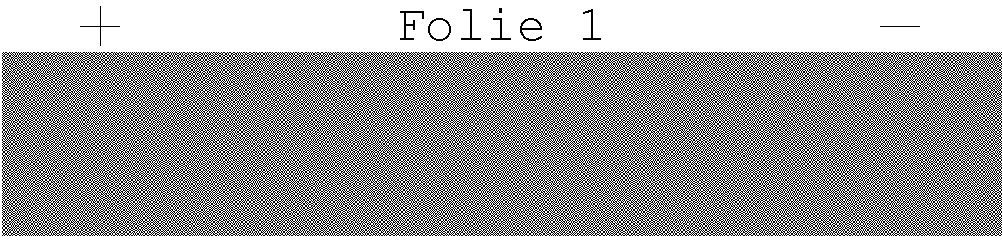
\includegraphics[width=1.\textwidth]{images/visual2.png}
			\caption{Eine zufällige erste Folie. Von \cite{visual}.}
			\label{sheet1}
		\end{figure}
		
		Die Pixel der zweiten Folie (Abbildung \ref{sheet2}) werden gemäß Abbildung \ref{generation-of-2nd-sheet} berechnet. Wenn im Original ein schwarzes Pixel ($ \blacksquare $) vorhanden ist, muss an dieser Stelle in der zweiten Folie das Komplement der ersten Folie eingefärbt werden. Somit sind bei Überlagerung beider Folien alle 4 Sub-Pixel schwarz. Wenn das originale Pixel weiß ist ($ \square $), hat das Quadrat der zweiten Folie das gleiche Muster wie die erste Folie. Das ergibt in Summe ein graues Pixel (\texttt{\#7F7F7F}). Weiße Pixel können über Folien nicht rekonstruiert werden, da mit den Folien keine Subtraktion möglich ist. Deshalb muss die Pixelanzahl auch vervierfacht werden. Siehe \cite{visual}.
		
		\begin{figure}[H]
			\centering
			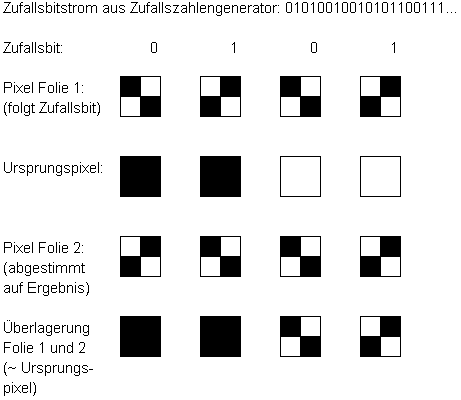
\includegraphics[width=0.6\textwidth]{images/visual1.png}
			\caption{Berechnung der Pixel der zweiten Folie. Von \cite{visual}.}
			\label{generation-of-2nd-sheet}
		\end{figure}
	
		\begin{figure}[H]
			\centering
			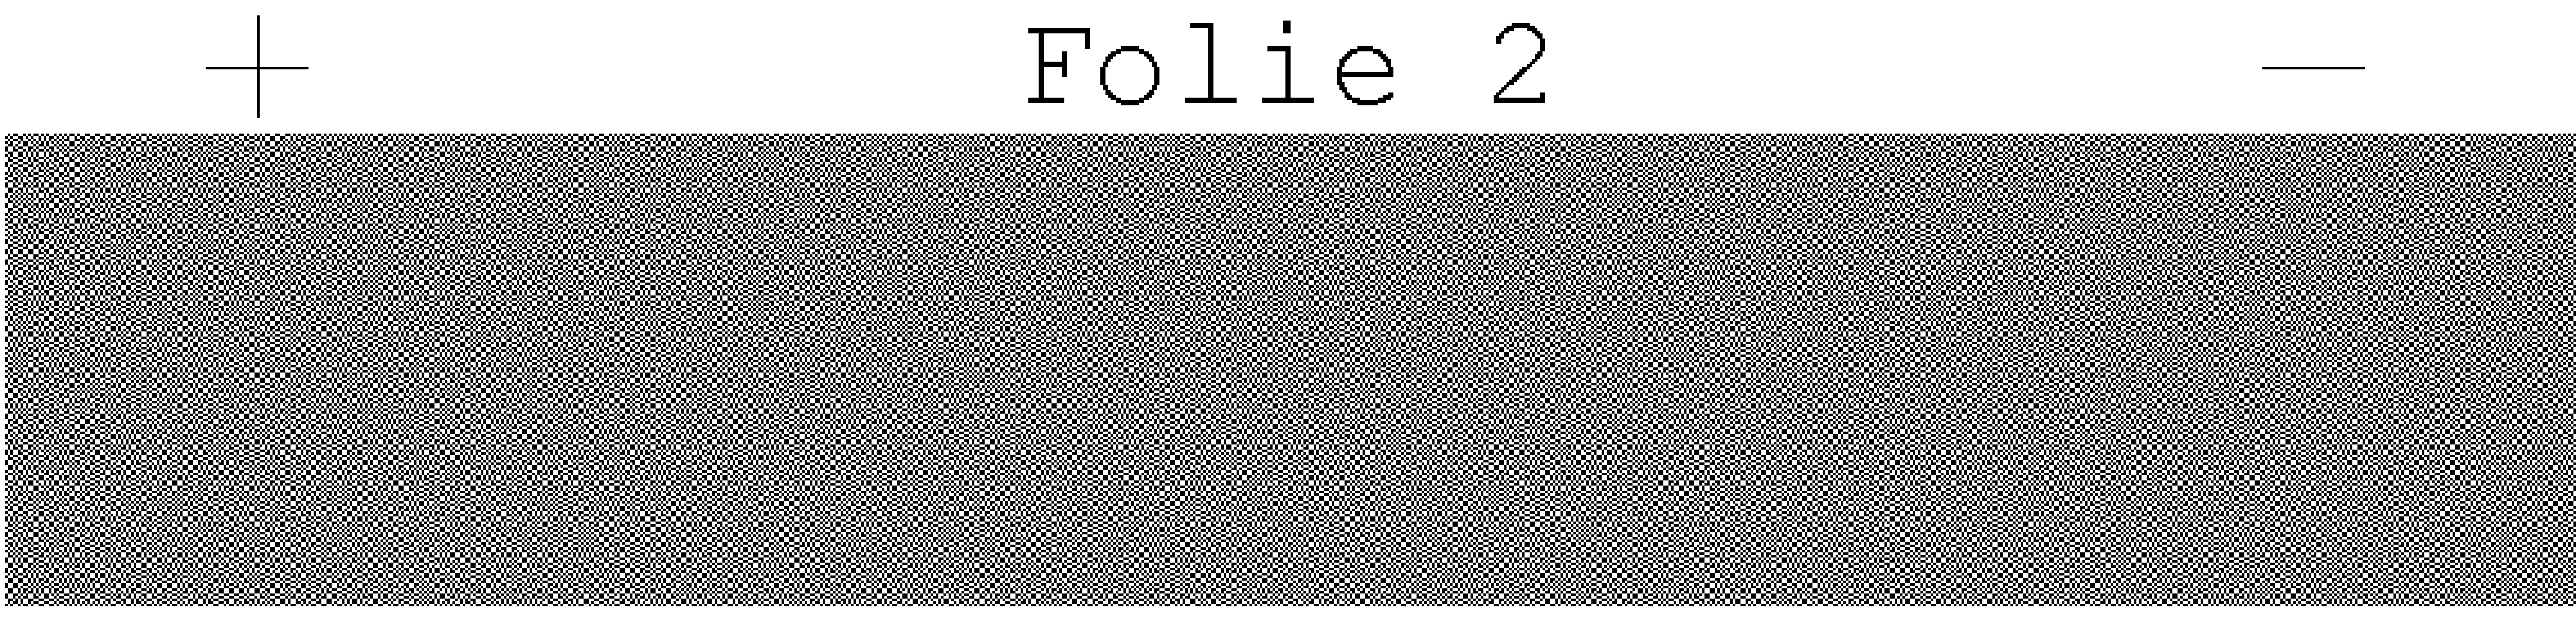
\includegraphics[width=1.\textwidth]{images/visual3.png}
			\caption{Die zweite Folie. Von \cite{visual}.}
			\label{sheet2}
		\end{figure}
	
		Wenn nun beide Folien übereinandergelegt werden, erscheint das Geheimnis:
		
		\begin{figure}[H]
			\centering
			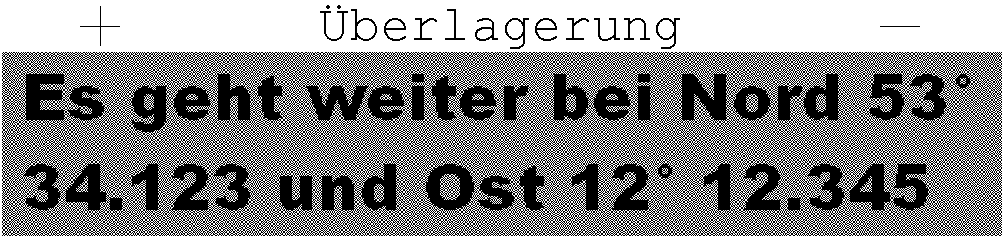
\includegraphics[width=1.\textwidth]{images/visual4.png}
			\caption{Das mittels beider Folien rekonstruierte Geheimnis. Von \cite{visual}.}
			\label{secret-image}
		\end{figure}
	\end{bsp}
	
	\subsubsection{One-Time-Padding mit mehr als 2 Personen}
	Wie sieht es jedoch aus, wenn sich mehr als zwei Personen ein Geheimnis mittels OTP\footnote{One-Time-Padding} teilen möchten? Auch dies ist möglich für eine beliebige Anzahl $ N $ an Personen. Doch was passiert, wenn einer der Beteiligten den eigenen Share verliert? Da alle Shares benötigt werden um $ D $ zu rekonstruieren, ist das unser SPOF\footnote{Single Point of Failure}. Da dies in der Praxis für große $ N $ sehr schnell zu einem Problem führen kann, möchten wir dieses Verfahren hier nicht länger behandeln.
	
	\section{Shamir's Secret Sharing}
	
	Wir widmen uns nun einem Verfahren mit dem sich ein Geheimnis rekonstruieren lässt, ohne dass alle Shares benötigt sind. Wie im Beispiel mit den Schlössern wollen wir einen Schwellwert von Shares angeben, die mindestens zur Rekonstruktion des Geheimnisses benötigt sein sollen. Das hier vorgestellte Secret-Sharing-Protokoll stammt von Adi Shamir. \cite{shamir}
	
	Seien $ n, t \in \N $ mit $ t \leq n $. Bei diesem $ (n,t) $-Secret-Sharing-Protokoll wird das Geheimnis von einem Dealer auf $ n $ Personen aufgeteilt. Jeder hat einen Teil des Geheimnisses. Wenn sich $ t $ dieser Personen zusammentun, sollen sie das Geheimnis rekonstruieren können. Wenn sich aber weniger als $ t $ dieser Geheimnisträger zusammentun, sollen sie keine relevante Information über das Geheimnis erhalten können. \cite{buchmann}
	
	Das Verfahren beruht auf der Interpolation von Lagrange für Polynome. Haben wir $ k $ verschiedene Punkte in einem zweidimensionalen Koordinatensystem $ (x_1, y_1), \dots (x_k, y_k) $ gegeben, wobei die $ x_i $ paarweise verschieden sind, folgt nach dem Fundamentalsatz der Algebra, dass es genau ein Polynom $ q(x) $ vom Grad $ k - 1 $ gibt, sodass $ q(x) =y_i $ für alle $ i $. \cite{shamir}
	
	\subsection{Die Vandermonde-Matrix}
	
	Bevor wir mit der Beschreibung des Protokolls beginnen können, beschäftigen wir uns mit \emph{Vandermonde\footnote{nach Alexandre-Théophile Vandermonde}-Matrizen}.
	
	\begin{def1}
		Eine Vandermonde-Matrix $ V_n $ ist eine $ (n \times n) $-Matrix der Form
	$$V_n =
	\begin{pmatrix}
	1 & a_1 & a_1^2 & \cdots & a_1^{n-1} \\
	1 & a_2 & a_2^2 & \cdots & a_2^{n-1} \\
	\vdots & \vdots & \vdots & \ddots & \vdots \\     
	1 & a_n & a_n^2 & \cdots & a_n^{n-1}
	\end{pmatrix}.$$
	Hierbei gilt $V_n = V(a_1, \dots, a_n) := (v_{ij}) $ mit $ v_{ij} := a_i^{(j-1)} $ für $ 1 \leq i, j \leq n$.
	\end{def1}
	\begin{satz}
		Die Determinante einer Vandermonde-Matrix $ V_n $ ist
		$$ \det V_n = \prod_{1 \leq j < i \leq n} (a_i - a_j). $$
	\end{satz}

	\begin{bew}
		Wir beweisen dies mithilfe vollständiger Induktion. \cite{vandermonde} Den trivialen Fall für $ \det V_1 = \det \begin{pmatrix}1\end{pmatrix} = 1 $ vernachlässigen wir hierbei.
		
		\begin{itemize}
			\item {\underline{\textbf{Induktionsanfang $ n=2 $:}}
				
				Der Induktionsanfang für $ n=2 $ ist schnell gezeigt:
				$$ \det (V_2) = \begin{vmatrix}1&a_1\\1&a_2\end{vmatrix} = 1 \cdot a_2 - 1 \cdot a_1 = \prod_{j=1, i=2} (a_i-a_j) = \prod_{1 \leq j < i \leq 2} (a_i-a_j).$$
			}
			\item {\underline{\textbf{Induktionsschritt $ n - 1 \rightarrow n $:}}
				
				Wir wollen dies mithilfe der Entwicklung nach Zeilen oder Spalten zeigen. Da sich dies nur empfiehlt, wenn möglichst viele Nullen in einer Zeile oder Spalte stehen, versuchen wir dies mithilfe elementarer Umformungen zu erreichen.
				
				Sei $$ \det V_n =
				\begin{vmatrix}
				1 & a_1 & a_1^2 & \cdots & a_1^{n-1} \\
				1 & a_2 & a_2^2 & \cdots & a_2^{n-1} \\
				\vdots & \vdots & \vdots & \ddots & \vdots \\     
				1 & a_n & a_n^2 & \cdots & a_n^{n-1}
				\end{vmatrix}.$$
%				Wenn wir nun die erste Zeile von allen anderen subtrahieren, stehen in der ersten Spalte nur noch eine Eins und sonst Nullen:
%				$$ \begin{vmatrix}
%				1 & a_1 & a_1^2 & \cdots & a_1^{n-1} \\
%				1 & a_2 & a_2^2 & \cdots & a_2^{n-1} \\
%				\vdots & \vdots & \vdots & \ddots & \vdots \\     
%				1 & a_n & a_n^2 & \cdots & a_n^{n-1}
%				\end{vmatrix} = 
%				\begin{vmatrix}
%				1 & a_1 & a_1^2 & \cdots & a_1^{n-1} \\
%				0 & a_2 - a_1 & a_2^2 - a_1^2 & \cdots & a_2^{n-1} - a_1^{n-1} \\
%				\vdots & \vdots & \vdots & \ddots & \vdots \\     
%				0 & a_n - a_1 & a_n^2 - a_1^2 & \cdots & a_n^{n-1} - a_1^{n-1}
%				\end{vmatrix}.$$
%				Jetzt entwickeln wir nach der ersten Spalte. Dann erhalten wir:
%				$$ \ldots = \begin{vmatrix}
%				a_2 - a_1 & a_2^2 - a_1^2 & \cdots & a_2^{n-1} - a_1^{n-1} \\
%				\vdots & \vdots & \ddots & \vdots \\     
%				a_n - a_1 & a_n^2 - a_1^2 & \cdots & a_n^{n-1} - a_1^{n-1}
%				\end{vmatrix}.$$
%				Diese Matrix ist leider noch keine Vandermonde-Matrix.
				Um in der ersten Zeile möglichst viele Nullen zu bekommen, subtrahieren wir zunächst das $ a_1 $-fache der $ (n-1) $-ten Spalte von der $ n $-ten Spalte, dann das $ a_1 $-fache der $ (n-2) $-ten Spalte von der $ (n-1) $-ten Spalte und so weiter bis wir das $ a_1 $-fache der ersten Spalte von der zweiten subtrahieren. Damit erhalten wir:
				$$ \ldots = 
				\begin{vmatrix}
				1 & 0 & 0 & \cdots & 0 \\
				1 & a_2 - a_1 & a_2^2 - a_1 \cdot a_2 & \cdots & a_2^{n-1} - a_1 \cdot a_2^{n-2} \\
				\vdots & \vdots & \vdots & \ddots & \vdots \\     
				1 & a_n - a_1 & a_n^2 - a_1 \cdot a_n & \cdots & a_n^{n-1} - a_1 \cdot a_n^{n-2}
				\end{vmatrix}.$$
				Dies ist noch keine Vandermonde-Matrix. Wenn wir jedoch folgende Umformung vornehmen, kommen wir unserem Ziel näher:
				$$ \ldots = 
				\begin{vmatrix}
				1 & 0 & 0 & \cdots & 0 \\
				1 & (a_2 - a_1) \cdot 1 & (a_2 - a_1) \cdot a_2 & \cdots & (a_2 - a_1) \cdot a_2^{n-2} \\
				\vdots & \vdots & \vdots & \ddots & \vdots \\     
				1 & (a_n - a_1) \cdot 1 & (a_n - a_1) \cdot a_n & \cdots & (a_n - a_1) \cdot a_n^{n-2}
				\end{vmatrix}.$$
				Jetzt entwickeln wir nach der ersten Spalte und erhalten:
				$$ \ldots = \begin{vmatrix}
				(a_2 - a_1) & (a_2 - a_1) \cdot a_2 & \cdots & (a_2 - a_1) \cdot a_2^{n-2} \\
				\vdots & \vdots & \ddots & \vdots \\     
				(a_n - a_1) & (a_n - a_1) \cdot a_n & \cdots & (a_n - a_1) \cdot a_n^{n-2}
				\end{vmatrix}.$$
				Jetzt ziehen wir die Faktoren aus der Determinante heraus und bekommen:
				$$ \ldots = (a_2 - a_1) \cdot \ldots \cdot (a_n - a_1)
				\begin{vmatrix}
				1 & a_2 & \cdots & a_2^{n-2} \\
				\vdots & \vdots & \ddots & \vdots \\     
				1 & a_n & \cdots & a_n^{n-2}
				\end{vmatrix}.$$
				Die Matrix ist nun tatsächlich eine Vandermonde-Matrix auf die wir unsere Induktionsvoraussetzung anwenden dürfen. Achtung: Die Indizes beginnen erst bei 2! Für diese $ (n-1 \times n-1) $-Matrix gilt nach der Induktionsvoraussetzung:
				$$\begin{vmatrix}
				1 & a_2 & \cdots & a_2^{n-2} \\
				\vdots & \vdots & \ddots & \vdots \\     
				1 & a_n & \cdots & a_n^{n-2}
				\end{vmatrix}
				= \prod_{2 \leq j < i \leq n} (a_j-a_i).$$
				Daraus folgt für die Determinante einer Vandermonde-Matrix:
				\begin{alignat*}{2}
				V(a_1, \dots, a_n) = & \ldots = (a_2 - a_1) \cdot \ldots \cdot (a_n - a_1) \prod_{2 \leq j < i \leq n} (a_i - a_j)\\
				 = & \prod_{j=1, 1 < i \leq n} (a_i - a_j) \prod_{2 \leq j < i \leq n} (a_i - a_j)\\
				 = & \prod_{1 \leq j < i \leq n} (a_i - a_j).
				\end{alignat*}
			Damit haben wir auch den Induktionsschritt gezeigt.
			}
		\end{itemize}
	\end{bew}
	
	\subsection{Das Shamir-Secret-Sharing-Protokoll}
	Jetzt können wir mit der Beschreibung des Protokolls beginnen.
	
	\begin{satz}\label{multiple-polynoms-sentence}
		Seien $ l, t \in \N, l \leq t $. Weiter seien $ x_i, y_i \in \Z / p\Z, 1 \leq i \leq l $, wobei die $ x_i $ paarweise verschieden sind. Dann gibt es genau $ p^{t-l} $ Polynome $ b \in (\Z / p\Z)[X] $ vom Grad $ \leq t - 1 $ mit $ b(x_i) = y_i, 1 \leq i \leq l $, wobei $ p $ eine Primzahl ist.\footnote{In unserem konkreten Fall gilt $ l = t $.}
	\end{satz}
	\begin{bew}
		Das Lagrange-Interpolationsverfahren liefert das Polynom
		$$ b(x) = \sum_{i=1}^{l} y_i \prod_{j=1, j \neq i}^{l} \frac{x_j - X}{x_j - x_i}, $$
		das $ b(x_i) = y_i, 1 \leq i \leq l $ erfüllt und mit dem sich $ b $ wieder interpolieren lässt. Jetzt muss nur noch die Anzahl dieser Polynome bestimmt werden.
		
		Sei $ b \in (\Z / p\Z)[X] $ ein solches Polynom. Dieses lässt sich wie folgt darstellen:
		$$ b(x) = \sum_{j=0}^{t-1} b_j X^j, b_j \in \Z / p\Z, 0 \leq j \leq t-1. $$
		Aus $ b(x_i) = y_i, 1 \leq i \leq l $ erhält man das lineare Gleichungssystem
		\begin{equation}\label{linear-equation-system}
			\begin{pmatrix}
			1 & x_1 & x_1^2 & \cdots & x_1^{t-1} \\
			1 & x_2 & x_2^2 & \cdots & x_2^{t-1} \\
			\vdots & \vdots & \vdots & \ddots & \vdots \\     
			1 & x_l & x_l^2 & \cdots & x_l^{t-1}
			\end{pmatrix}
			\begin{pmatrix}
			b_0 \\
			b_1 \\
			\vdots \\     
			b_{t-1}
			\end{pmatrix}
			=
			\begin{pmatrix}
			y_1 \\
			y_2 \\
			\vdots \\     
			y_l
			\end{pmatrix}.
		\end{equation}		
		Die Teil-Koeffizientenmatrix
		$$ U =
		\begin{pmatrix}
		1 & x_1 & x_1^2 & \cdots & x_1^{l-1} \\
		1 & x_2 & x_2^2 & \cdots & x_2^{l-1} \\
		\vdots & \vdots & \vdots & \ddots & \vdots \\     
		1 & x_l & x_l^2 & \cdots & x_l^{l-1}
		\end{pmatrix} $$
		ist eine Vandermonde-Matrix. Ihre Determinante ist
		$$ \det U = \prod_{1 \leq j < i \leq l} (x_i-x_j). $$
		Weil die $ x_i $ nach Voraussetzung paarweise verschieden sind, ist die Determinante ungleich Null. Der Rang von $ U $ ist also $ l $. Daher hat der Kern der Koeffizientenmatrix des linearen Gleichungssystems (\ref{linear-equation-system}) den Rang $ t-l $ und die Anzahl der Lösungen ist $ p^{t-l} $.
	\end{bew}
	
	\subsection{Berechnung der Shares}
	
	Der Dealer wählt eine Primzahl $ p, p \geq n + 1 $ und paarweise von Null verschiedene Elemente $ x_i \in \Z / p \Z, 1 \leq i \leq n $. Die Elemente aus $ \Z / p \Z $ stellen wir hier durch ihre kleinsten nicht negativen Vertreter dar. Die $ x_i $ werden veröffentlicht.
	
	Ein Geheimnis $ s \in \Z / p \Z $ will vom Dealer verteilt werden. Dabei wird wie folgt vorgegangen:
	
	\begin{enumerate}
		\item {
			Der Dealer wählt geheime Elemente $ a_j \in \Z / p \Z, 1 \leq j \leq t - 1 $ und konstruiert daraus das Polynom a(X), dessen Grad $ \leq t-1 $:
			\begin{equation}\label{secret-polynom-to-reconstruct}
			a(x) = s + \sum_{j=1}^{t-1} a_jX^j.
			\end{equation}
		}
		\item {
			Nun werden die Shares berechnet: $ y_i = a(x_i), 1 \leq i \leq n $.
		}
		\item {
			Der $ i $-te Geheimnisträger erhält den Geheimnisteil $ y_i, 1 \leq i \leq n $.
		}
	\end{enumerate}
	Das Geheimnis ist der konstante Term $ a(0) $ des Polynoms $ a(X) $.
	\begin{bsp}\label{shares-example}
		Sei $ n = 5, t = 3 $. Der Dealer wählt $ p = 17, x_i = i, 1 \leq i \leq 5 $.
		
		Das Geheimnis sei $ s = 3 $. Als geheime Koeffizienten des Polynoms werden $ a_i = 13 + i, 1 \leq i \leq 2 $ gewählt. Wir erhalten das geheime Polynom:
		$$ a(x) = 15 X^2 + 14X + 3. $$
		Die Geheimnisteile sind also:
		$$\begin{array}{cccccc}
			y_1 & = & a(1) & = & 15 & , \\
			y_2 & = & a(2) & = & 6 & , \\
			y_3 & = & a(3) & = & 10 & , \\
			y_4 & = & a(4) & = & 10 & , \\
			y_5 & = & a(5) & = & 6 & .
		\end{array}$$
	\end{bsp}
	
	\subsection{Rekonstruktion des Geheimnisses}
	
	Angenommen, es arbeiten $ t $ Geheimnisträger zusammen. Die Shares seien $ y_i = a(x_i), 1 \leq i \leq t $. Hierbei ist $ a(X) $ das Polynom aus (\ref{secret-polynom-to-reconstruct}). Dies kann man durch Umnummerierung der Geheimnisteile immer erreichen. Jetzt gilt
	$$ a(X) = \sum_{i=1}^{t} y_i \prod_{j=1, j \neq i}^{t} \frac{x_j - X}{x_j - x_i} . $$
	Dieses Polynom erfüllt nämlich $ a(x_i) = y_i, 1 \leq i \leq t $ und nach Satz \ref{multiple-polynoms-sentence} gibt es genau ein solches Polynom vom Grad höchstens $ t - 1 $. Daher ist
	\begin{equation}\label{formula-to-insert-shares-to}
		s = a(0) = \sum_{i=1}^{t} y_i \prod_{j=1, j \neq i}^{t} \frac{x_j}{x_j - x_i} .
	\end{equation}
	Die Formel (\ref{formula-to-insert-shares-to}) wird von den Geheimnisträgern benutzt, um das Geheimnis zu rekonstruieren.
	\pagebreak
	\begin{bsp}
		Wir setzen das Beispiel \ref{shares-example} fort.

		Die ersten drei Geheimnisträger rekonstruieren das Geheimnis. Mithilfe der Lagrange-Interpolationsformel erhalten wir:		
		\begin{alignat*}{2}
		a(0) & = & & \sum_{i=1}^{t} y_i \prod_{j=1, j \neq i}^{t} \frac{x_j}{x_j - x_i} \\
		       & = & & y_1  \left( \frac{x_2}{x_2 - x_1} \cdot \frac{x_3}{x_3 - x_1} \right) \\
		        &   & + &  y_2  \left( \frac{x_1}{x_1 - x_2} \cdot \frac{x_3}{x_3 - x_2} \right) \\
				&  &  + & y_3  \left( \frac{x_1}{x_1 - x_3} \cdot \frac{x_2}{x_2 - x_3} \right) \\
		& =&& 15 \left( \frac{2}{2 - 1} \cdot \frac{3}{3 - 1} \right) 
		+  6  \left( \frac{1}{1 - 2} \cdot \frac{3}{3 - 2} \right) 
		+ 10  \left( \frac{1}{1 - 3} \cdot \frac{2}{2 - 3} \right)\\
		&=&& 15 \frac{6}{2} + 6 \frac{3}{-1} + 10 \frac{2}{2} = 37 \bmod 17 = 3.
		\end{alignat*}
%		$$
%			\begin{array}{rccl}
%			a(0) & = & & \sum_{i=1}^{t} y_i \prod_{j=1, j \neq i}^{t} \frac{x_j}{x_j - x_i} \\
%			& = & & y_1  \left( \frac{x_2}{x_2 - x_1} \cdot \frac{x_3}{x_3 - x_1} \right) \\
%			&   & + &  y_2  \left( \frac{x_1}{x_1 - x_2} \cdot \frac{x_3}{x_3 - x_2} \right) \\
%			&  &  + & y_3  \left( \frac{x_1}{x_1 - x_3} \cdot \frac{x_2}{x_2 - x_3} \right) \\
%			& =&& 15 \left( \frac{2}{2 - 1} \cdot \frac{3}{3 - 1} \right) 
%			+  6  \left( \frac{1}{1 - 2} \cdot \frac{3}{3 - 2} \right) 
%			+ 10  \left( \frac{1}{1 - 3} \cdot \frac{2}{2 - 3} \right)\\
%			&=&& 15 \frac{6}{2} + 6 \frac{3}{-1} + 10 \frac{2}{2} = 37 \bmod 17 = 3.
%			\end{array}
%		$$
% TODO: Lösung für alignment finden!!!
	\end{bsp}
	
	\subsection{Sicherheit des Verfahrens}
	
	Angenommen, weniger als $ t $ Geheimnisträger versuchen gemeinsam, das Geheimnis $ s $ zu ermitteln. Ihre Anzahl sei $ m, m < t $. Ihre Geheimnisteile seien $ y_i, 1 \leq i \leq m $. Die Geheimnisträher wissen, dass das Geheimnis der konstante Term eines Polynoms $ a \in \Z_p[X] $ vom Grad $ \leq t - 1 $ ist, das $ a(x_i) = y_i, 1 \leq i \leq m $ erfüllt. Aus Satz \ref{multiple-polynoms-sentence} erhält man das folgende Resultat:
	
	\begin{lemma}\label{lemma-multiple-possibilities}
		Für jedes $ s' \in \Z / p \Z $ gibt es genau $ p^{t-m-1} $ Polynome $ a'(X) \in (\Z / p \Z)[X] $ vom Grad $ \leq t - 1 $ mit $ a'(0) = s' $ und $ a'(x_i) = y_i, 1 \leq i \leq m $.
	\end{lemma}

	\begin{bew}
		Da die $ x_i $ paarweise und von Null verschieden sind, folgt die Behauptung aus Satz \ref{multiple-polynoms-sentence} mit $ l = m + 1 $.
	\end{bew}

	Lemma \ref{lemma-multiple-possibilities} zeigt, dass die $ m $ Geheimnisträger keine Information über das Geheimnis bekommen, weil alle mögliche konstanten Terme gleich wahrscheinlich sind.
	\subsection{Graphische Beispiele}
		Das Verfahren kann auch graphisch dargestellt werden. Es folgen Beispiele \ref{bsp:graph-1} und \ref{bsp:graph-2}: TBC\dots % TODO Elaborate on examples
		\pagebreak
		\subsubsection{Graphisches \texorpdfstring{$ (2,n) $}{(2,n)}-Schema}
		\begin{bsp}\label{bsp:graph-1}
		TBC\dots % TODO (2,n) $-Schema
		
		\begin{figure}[H]
			\begin{adjustbox}{center}
				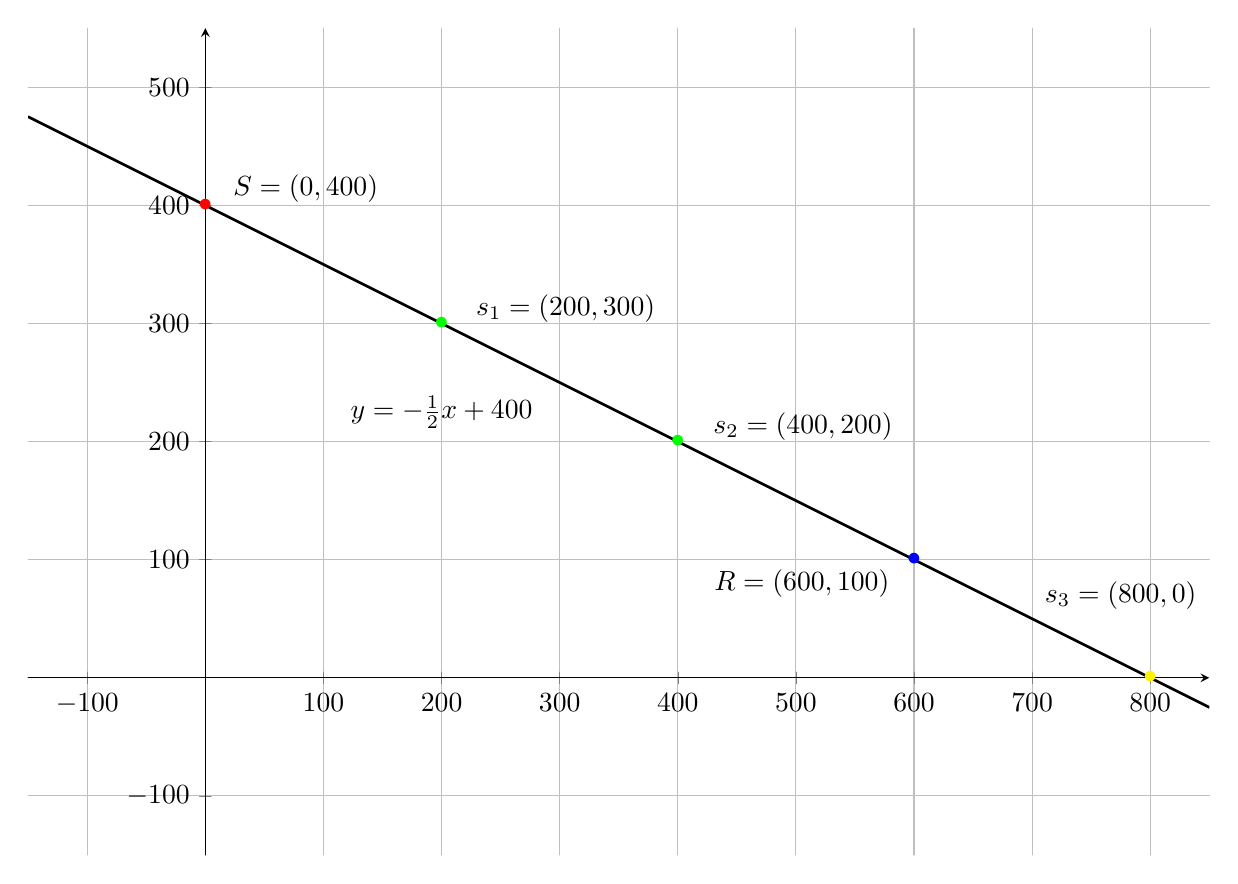
\begin{tikzpicture}[line cap=round,line join=round,>=triangle 45,x=0.015cm,y=0.015cm]
				\begin{axis}[x=0.015cm,y=0.015cm,axis lines=middle,ymajorgrids=true,xmajorgrids=true,
				xmin=-150.,xmax=850.,xtick={-100.,0.,...,850.},
				ymin=-150.,ymax=550.,ytick={-100.,0.,...,550.},]
				\clip(-150.,-150.) rectangle (850.,550.);
				\draw [line width=1.pt,domain=-150.:850.] plot(\x,{(--240000.-300.*\x)/600.});
				\draw (200.,225.) node {$y=-\frac{1}{2}x+400$};
				\draw[color=red] (0.,400.) node {$ \bullet $};
				\draw (85.,414.) node {$S=(0,400)$};
				\draw[color=blue] (600.,100.) node {$ \bullet $};
				\draw (505.,80.) node {$R=(600,100)$};
				\draw[color=green] (200.,300.) node {$ \bullet $};
				\draw (305.,313.) node {$s_1=(200,300)$};
				\draw[color=green] (400.,200.) node {$ \bullet $};
				\draw (506.,213.) node {$s_2=(400,200)$};
				\draw[color=yellow] (800.,0.) node {$ \bullet $};
				\draw (775.,70.) node {$s_3=(800,0)$};
				\end{axis}
				\end{tikzpicture}
			\end{adjustbox}
			\caption{Erweiterung des Geheimnisses $ S $ als Gerade $ f $ für zwei Shares $s_1$ und $s_2$.} % TODO Caption
		\end{figure}
	\end{bsp}
	\pagebreak
	\subsubsection{Graphisches \texorpdfstring{$ (3,n) $}{(3,n)}-Schema}
	\begin{bsp}\label{bsp:graph-2}
		TBC\dots % TODO (3,n) $-Schema
		
		\begin{figure}[H]
			\begin{adjustbox}{center}
				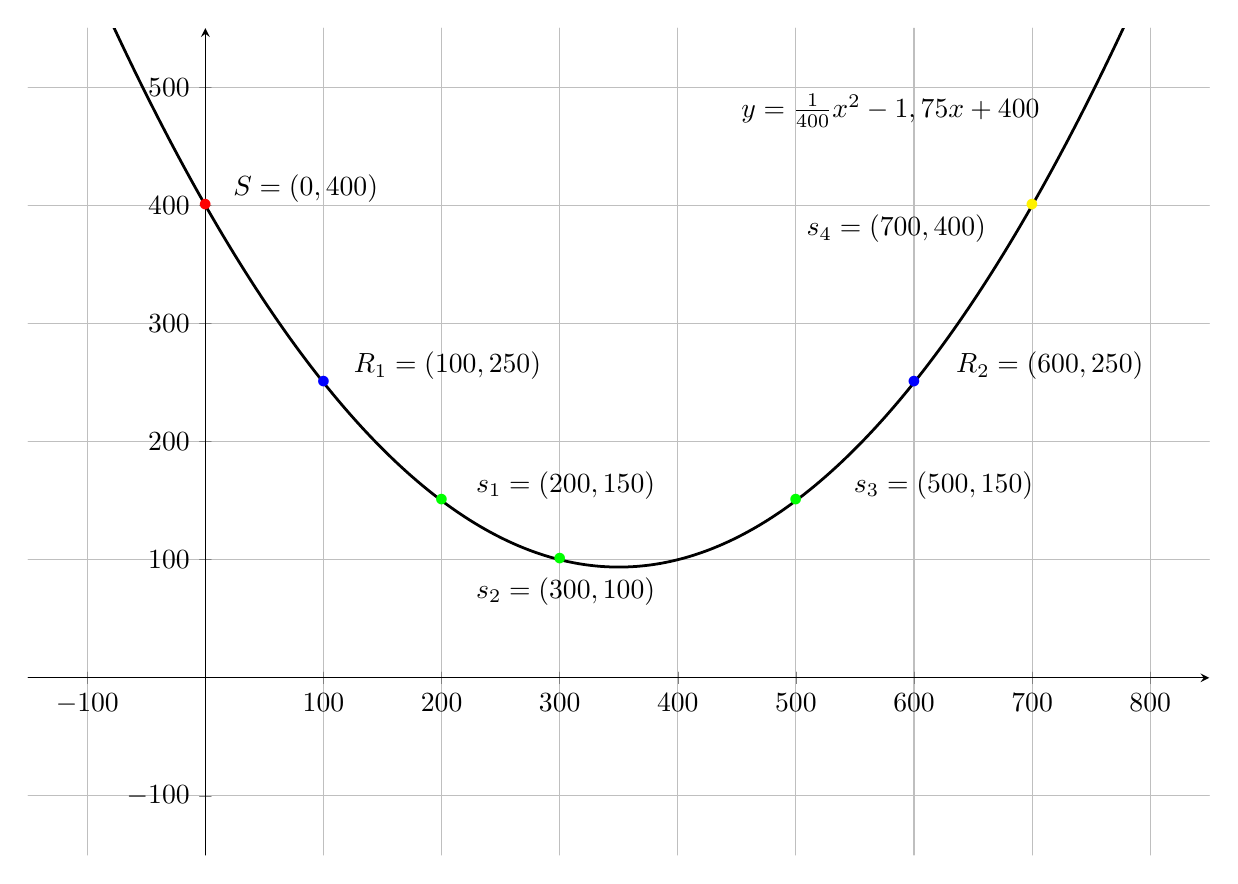
\begin{tikzpicture}[line cap=round,line join=round,>=triangle 45,x=0.015cm,y=0.015cm]
				\begin{axis}[x=0.015cm,y=0.015cm,axis lines=middle,ymajorgrids=true,xmajorgrids=true,
				xmin=-150.,xmax=850.,xtick={-100.,0.,...,850.},
				ymin=-150.,ymax=550.,ytick={-100.,0.,...,550.},]
				\clip(-150.,-150.) rectangle (850.,550.);
				\draw[line width=1.pt,smooth,samples=100,domain=-150.0:850.0] plot(\x,{0.0025*(\x)^(2.0)-1.75*(\x)+400.0});
				\draw[color=red] (0.,400.) node {$ \bullet $};
				\draw (85.,414.) node {$S=(0,400)$};
				\draw[color=blue] (100.,250.) node {$ \bullet $};
				\draw (205.,264.) node {$R_1=(100,250)$};
				\draw[color=blue] (600.,250.) node {$ \bullet $};
				\draw (715.,264.) node {$R_2=(600,250)$};
				\draw (580.,480.) node {$y=\frac{1}{400}x^2-1,75x+400$};
				\draw[color=green] (200.,150.) node {$ \bullet $};
				\draw (305.,163.) node {$s_1=(200,150)$};
				\draw[color=green] (300.,100.) node {$ \bullet $};
				\draw (305.,73.) node {$s_2=(300,100)$};
				\draw[color=green] (500.,150.) node {$ \bullet $};
				\draw (625.,163.) node {$s_3=(500,150)$};
				\draw[color=yellow] (700.,400.) node {$ \bullet $};
				\draw (585.,380.) node {$s_4=(700,400)$};
				\end{axis}
				\end{tikzpicture}
			\end{adjustbox}
			\caption{Parabel} % TODO Caption
		\end{figure}
	\end{bsp}

	\subsection{Blakley's Secret-Sharing als weiteres Verfahren}
		% TODO Blakley's
		
		Blakley's Secret-Sharing-Protokoll hingegen basiert auf Projektiven Räumen. Der Dealer verteilt ein Geheimnis, einen Punkt, in diesem Raum, der die Dimension $ k $ hat. Jeder der $ n $ Personen erhält einen Teil des Raumes der Dimension $ k-1 $, beispielsweise eine Hyperebene. Im Raum $ \R^3 $ schneiden sich zwei nicht parallele Geraden, die in einer gemeinsamen Ebene liegen, in genau einem Punkt. Drei nicht parallele Ebenen schneiden sich im Raum in genau einem Punkt. Siehe Abbildung (\ref{bsp:blackley}). Allgemein schneiden sich $ n $ nicht parallele $ (n-1) $-dimensionale Hyperebenen in genau einem Punkt. Wenn nun $ k $ Personen Ihre Hyperebenen schneiden, erhalten sie das Geheimnis. \cite{blakley}\cite{quantum}
		\begin{figure}[H]
			\centering
			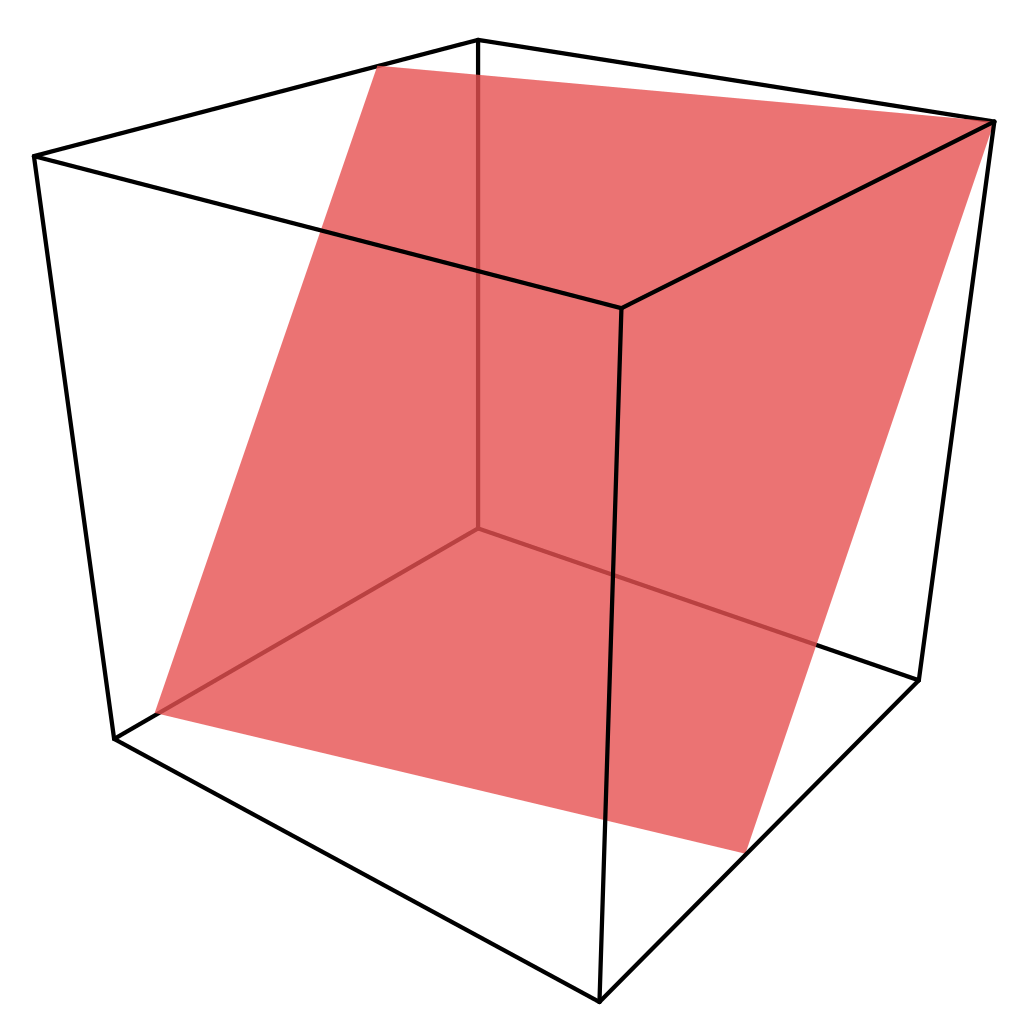
\includegraphics[width=0.3\textwidth]{images/blakley1.png}
			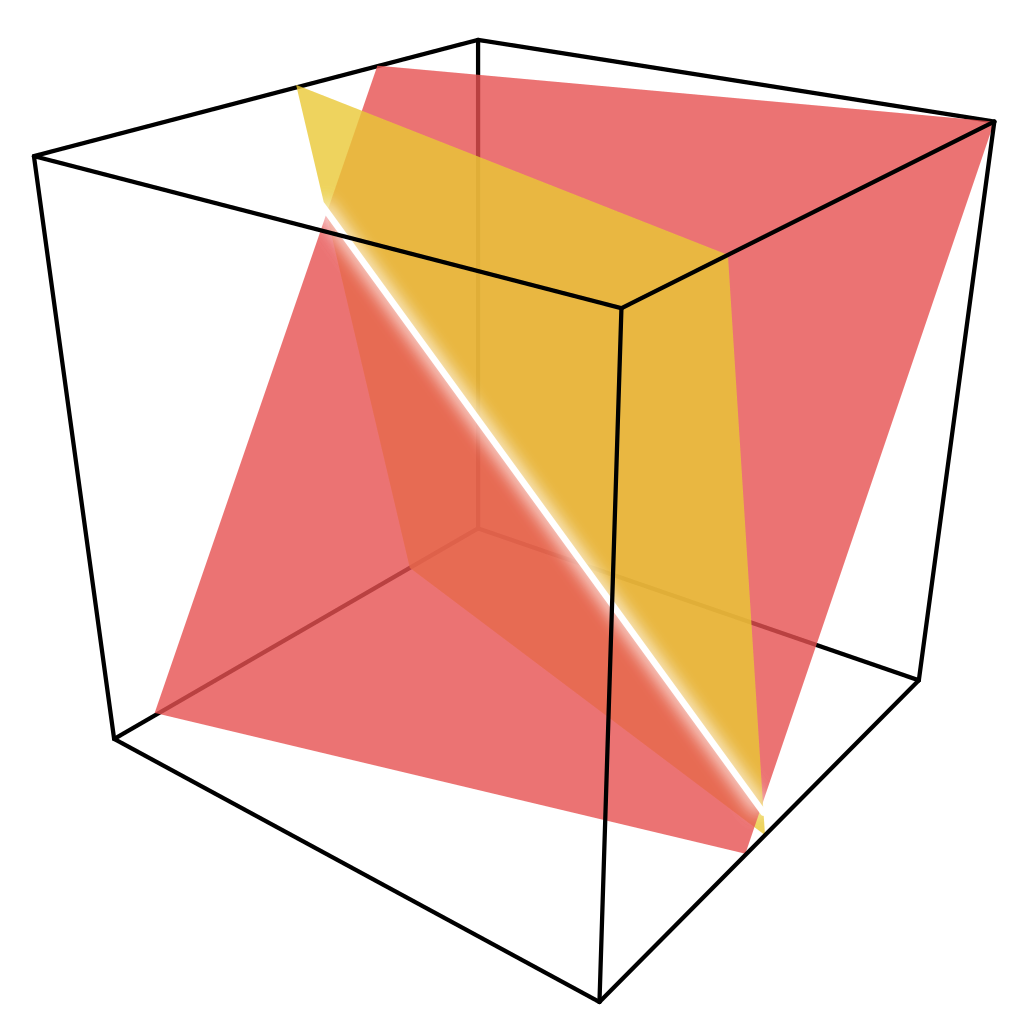
\includegraphics[width=0.3\textwidth]{images/blakley2.png}
			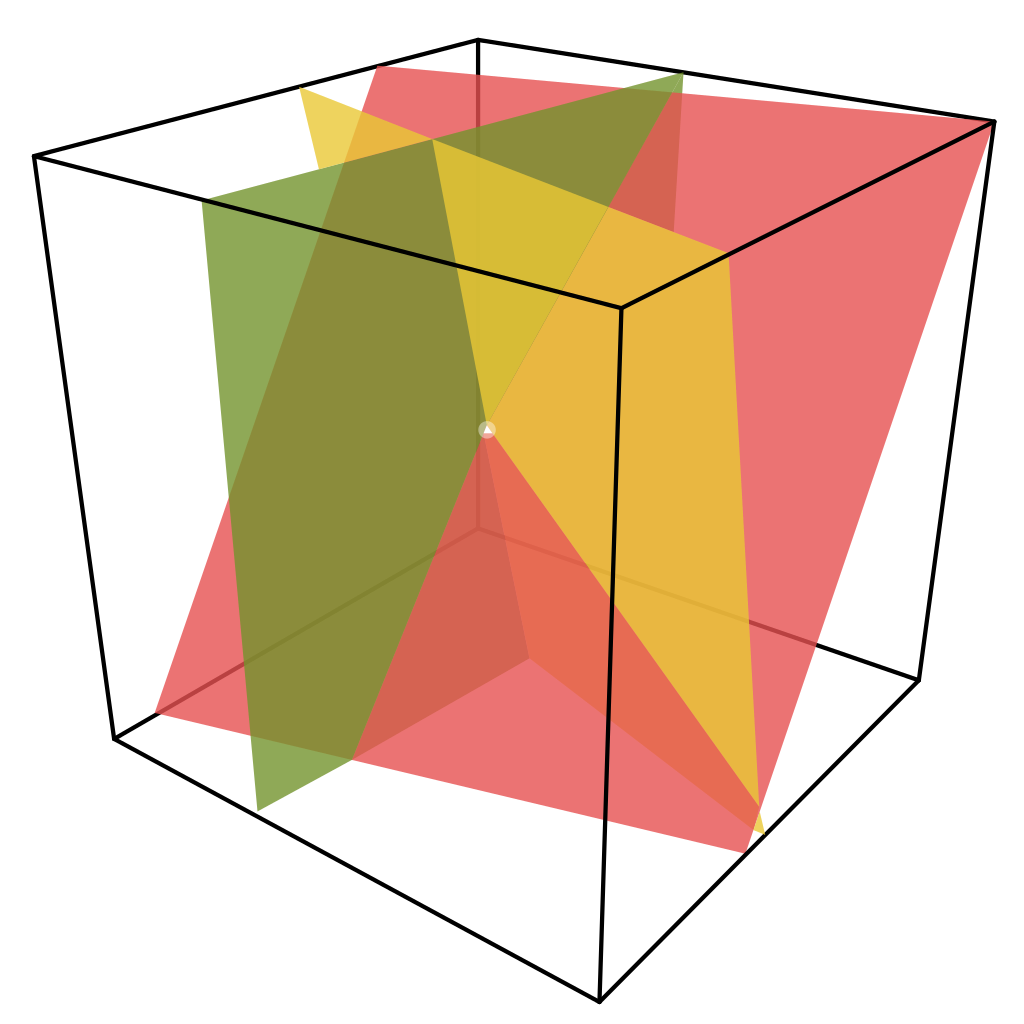
\includegraphics[width=0.3\textwidth]{images/blakley3.png}
			\caption{Blakley's Verfahren im $ \R^3 $: Jeder Share ist eine Ebene. Das Geheimnis ist der Punkt, in dem sich die drei Ebenen schneiden. Zwei Ebenen reichen nicht aus. Von \cite{blakley-images}.}
			\label{bsp:blackley}
		\end{figure}
		Bei Blakley's Schema nehmen die Shares mehr Platz in Anspruch. Bei Shamir sind die Shares nicht größer, als das Geheimnis selbst. Blakley's Shares sind $ t $-mal so groß. \cite{blakley}
	\section{Fazit}
	% TODO: Fazit
	Gegenüber dem eingangs gezeigten Beispiel mit den Schlüsseln und Schlössern bringt uns Shamir's Verfahren einige Vorteile:
	
	\begin{enumerate}
		\item {
			Die Größe jedes einzelnen Shares übersteigt nicht das Geheimnis.
		}
		\item {
			Wenn unser Schwellwert gleich bleibt, können wir nach Belieben Shares hinzufügen oder löschen, ohne die anderen Shares zu beeinflussen. Voraussetzung ist hier, dass es möglich sein muss, einzelne Shares vollständig zu löschen.
		}
		\item {
			Es ist sehr einfach, alle Shares auszutauschen, ohne das Geheimnis ändern zu müssen. Wir brauchen nur ein neues Polynom $ a'(X) $ mit $ a'(0) := a(0) $.
		}
		\item {
			Dieses Verfahren ermöglicht es uns, eine Hierarchie der Geheimnisträger zu erhalten. Geben wir beispielsweise dem Firmeninhaber drei Shares, dem Vice-Präsidenten zwei Shares und jeder anderen Führungsperson einen Share, erlaubt es ein $ (3, n) $-Schema, die Befugnisse entsprechend der Rollen zu verteilen. \cite{shamir}
		}
	\end{enumerate}
	TBC$\dots$ % TODO: Fazit
	\cleardoublepage
%	\phantomsection
%	\addcontentsline{toc}{chapter}{Abbildungsverzeichnis}
%	\listoffigures
	\begingroup
	\let\clearpage\relax
	\phantomsection
	\addcontentsline{toc}{chapter}{Literaturverzeichnis}
	\bibliographystyle{acm} % siam, alpha, alphadin, ieeetr, plain, acm, abbrvdin
	\bibliography{secret-sharing}
	\endgroup
\end{document}
